\documentclass[runningheads]{llncs}

\usepackage[T1]{fontenc}
\usepackage[spanish,es-tabla]{babel}
\usepackage{amsmath,amssymb}
\usepackage{graphicx}
\usepackage{booktabs}
\usepackage{textcomp}
\usepackage{url}

% Nombres de la plantilla LNCS en español (babel los cambiaría a «Figura»)
\addto\captionsspanish{\def\abstractname{Resumen.}\def\figurename{Fig.}}
\def\keywordname{\textbf{Palabras clave:}}
\newcommand{\keywords}[1]{\par\addvspace\baselineskip\noindent\keywordname\enspace\ignorespaces#1}

% Símbolos que se escriben tal cual en el texto
\DeclareUnicodeCharacter{2212}{\textminus}
\DeclareUnicodeCharacter{2264}{\ensuremath{\leq}}
\DeclareUnicodeCharacter{2265}{\ensuremath{\geq}}
\DeclareUnicodeCharacter{2248}{\ensuremath{\approx}}
\DeclareUnicodeCharacter{2713}{\ensuremath{\checkmark}}
\DeclareUnicodeCharacter{03C7}{\ensuremath{\chi}}
\DeclareUnicodeCharacter{03C3}{\ensuremath{\sigma}}
\DeclareUnicodeCharacter{03B1}{\ensuremath{\alpha}}

\begin{document}

\title{Estimación de la calidad de transmisión con aprendizaje automático en la red DWDM ferroviaria Moscú-Kazánskaya – Riazán}
\titlerunning{QoT con aprendizaje automático en una red DWDM ferroviaria}
\author{Angel Luis Acosta González}
\authorrunning{A.~L. Acosta González}
\institute{Máster Universitario en Sistemas Inteligentes, Universidad de Salamanca}
\maketitle

\begin{abstract}
La calidad de transmisión (QoT) de los canales de una red DWDM ferroviaria suele verificarse una sola vez, en la fase de diseño, con un cálculo analítico del caso más desfavorable y márgenes fijos. Este trabajo evalúa si un modelo de aprendizaje automático entrenado con parámetros observables de los enlaces puede predecir si cada canal cumple el umbral BER ≤ 10\textsuperscript{−11} cuando la red se degrada. Se generaron 10 000 canales sintéticos de la red Moscú-Kazánskaya – Riazán con un modelo físico de transmisión que incluye envejecimiento, reparaciones y hielo, y se compararon una regresión logística, Random Forest y XGBoost en tres escenarios de información. Con la potencia recibida medida, los tres modelos alcanzan un AUC de 0,998 (≥ 0,996 en trayectos no vistos); los ensambles obtienen mayor F1 (0,947 frente a 0,931) y cometen menos errores (prueba de McNemar, p $<$ 0,001), aunque la regresión logística detecta más canales que no cumplen. La potencia recibida medida es la variable decisiva en la red simulada. La hipótesis se confirma con matices y debe contrastarse con datos medidos en la red real.
\keywords{redes ópticas DWDM \textperiodcentered{} calidad de transmisión \textperiodcentered{} aprendizaje automático \textperiodcentered{} Random Forest \textperiodcentered{} comunicaciones ferroviarias}
\end{abstract}


\section{Introducción y marco teórico}\label{sec:1}

Las redes de comunicaciones ferroviarias transportan servicios críticos para la seguridad de la circulación: señalización, telemando, voz operativa y datos de explotación. En los tramos troncales estas redes se construyen cada vez más sobre fibra óptica con multiplexación densa por división de longitud de onda (DWDM), que permite transportar decenas de canales por la misma fibra. Cada canal óptico debe cumplir un umbral de calidad de transmisión (\emph{quality of transmission}, QoT), expresado habitualmente como una tasa de error de bit (\emph{bit error rate}, BER) máxima o su factor Q equivalente.

El caso de estudio es la red primaria de comunicaciones del tramo Moscú-Kazánskaya – Riazán-1 (198,3 km), diseñada en un trabajo previo del autor~\cite{acosta2026tfg} como un anillo DWDM con canales de 10 Gbit/s sobre fibra G.652. En ese diseño la QoT se verificó con un modelo analítico aplicado una sola vez al tramo más desfavorable (108,9 km), con márgenes fijos y sin considerar la degradación de la red durante su explotación: envejecimiento de la fibra y de los amplificadores, empalmes añadidos en reparaciones o pérdidas por hielo, riesgos que el propio proyecto identifica en el trazado.

La estimación de la QoT con aprendizaje automático es un campo consolidado en redes troncales; Pointurier~\cite{pointurier2021} revisa sus técnicas y sus fuentes de inexactitud. Samadi et al.~\cite{samadi2017} propusieron su uso para la operación dinámica de redes WDM, y Rottondi et al.~\cite{rottondi2018} clasificaron canales como aceptables o no con Random Forest entrenado con datos sintéticos, con una exactitud cercana a 0,96 y unas 1000 muestras suficientes. Morais y Pedro~\cite{morais2018} compararon varios modelos y estimaron además el margen residual, y Kozdrowski et al.~\cite{kozdrowski2021} confirmaron con datos reales de dos redes DWDM que Random Forest y XGBoost son los clasificadores más precisos, aunque con clases muy desbalanceadas. Aladin et al.~\cite{aladin2020} observaron que la exactitud cae de más del 99~\% a un 85–89~\% cuando solo se usan unas pocas variables, y Allogba et al.~\cite{allogba2022} recomiendan evaluar con métricas más allá de la exactitud. Otros trabajos abordan la transferencia de modelos entre redes~\cite{yu2019}, la estimación en sistemas IM/DD como el de la red ferroviaria~\cite{igarashi2024} y el pronóstico con incertidumbre~\cite{dicicco2023}.

En la búsqueda bibliográfica realizada en Web of Science (septiembre de 2026) no se han encontrado trabajos que apliquen estas técnicas a redes ferroviarias regionales, con muchas estaciones de acceso, condiciones climáticas severas y equipos de detección directa. La pregunta de investigación es si un modelo de aprendizaje automático entrenado con parámetros observables de los enlaces puede predecir si cada canal cumple el umbral BER ≤ 10\textsuperscript{−11} en condiciones de degradación con más acierto que un modelo sencillo. La hipótesis es que un modelo de ensamble lo predice con mayor acierto que un modelo lineal. Para contrastarla se plantean cuatro objetivos: (1) construir un conjunto de datos de canales de la red con un modelo físico que incluya degradación; (2) entrenar y comparar modelos de ensamble con una regresión logística de referencia; (3) evaluar su acierto en canales y condiciones no vistos durante el entrenamiento; y (4) cuantificar el margen de diseño que podría ahorrarse sin incumplir el umbral. Este trabajo aborda los objetivos 1 a 3; el objetivo 4, que exige estimar el margen residual de cada canal~\cite{morais2018} con su incertidumbre~\cite{dicicco2023}, queda fuera de su alcance y se plantea como trabajo futuro.

Las aportaciones son: (i) un modelo físico de la red con degradación en explotación y un conjunto de datos reproducible; (ii) la comparación de tres modelos en tres escenarios de información con validación cruzada y una prueba estadística, incluida la evaluación en trayectos y condiciones no vistos; y (iii) la identificación de la variable que más aporta a la predicción. La sección~\ref{sec:2} describe los métodos, la sección~\ref{sec:3} presenta y discute los resultados y la sección~\ref{sec:4} recoge las conclusiones.


\section{Métodos}\label{sec:2}


\subsection{Modelo físico de transmisión}

Cada canal une dos de las 21 estaciones de la línea, a una distancia \emph{d} de entre 5,4 y 198,3 km (208 pares posibles; se omite una estación cuyo punto kilométrico no consta en~\cite{acosta2026tfg}), y transmite 10 Gbit/s en formato sin retorno a cero (NRZ) con detección directa. La pérdida nominal del canal es la suma de la atenuación de la fibra (α = 0,22 dB/km), un empalme de 0,1 dB cada 4 km, 1 dB de conectores y 5 dB de los multiplexores de inserción-extracción (OADM), aplicados por igual a todos los canales:

\begin{equation}
L_{\mathrm{nom}} = \alpha d + 0{,}1\left\lceil d/4 \right\rceil + 1 + 5 \quad [\mathrm{dB}]
\label{eq:1}
\end{equation}

Con un láser de 0 dBm y una sensibilidad del receptor de −25 dBm, el canal se diseña con preamplificador de fibra dopada con erbio (EDFA) cuando el margen nominal es inferior a 3 dB, lo que ocurre en los canales de más de 65 km; los canales amplificados llevan un EDFA cada 110 km como máximo (\emph{n} vanos iguales), y \emph{P}\textsubscript{rx} = \emph{P}\textsubscript{tx} − \emph{L}/\emph{n} es la potencia a la entrada de cada amplificador o del receptor. En los canales sin amplificar, limitados por el ruido térmico del receptor, el factor Q crece de forma lineal con la potencia recibida \emph{P}\textsubscript{rx}, con Q = 7,03 en la sensibilidad (BER = 10\textsuperscript{−12}):

\begin{equation}
Q_t = 7{,}03 \cdot 10^{(P_{\mathrm{rx}} + 25)/10}
\label{eq:2}
\end{equation}

En los amplificados domina el ruido de emisión espontánea amplificada (ASE). La relación señal/ruido óptica en 0,1 nm y el factor Q con detección directa se obtienen como:

\begin{equation}
\mathrm{OSNR} = 58 + P_{\mathrm{rx}} - \mathrm{NF} - 10\log_{10} n \quad [\mathrm{dB}]
\label{eq:3}
\end{equation}

\begin{equation}
Q_{\mathrm{ASE}} = \sqrt{\frac{B_o}{B_e}}\,\frac{2\,\mathrm{OSNR}}{1 + \sqrt{1 + 4\,\mathrm{OSNR}}}
\label{eq:4}
\end{equation}

donde NF es la figura de ruido del EDFA (6–7 dB más su envejecimiento), B\textsubscript{o} = 12,5 GHz y B\textsubscript{e} = 7,5 GHz. El ruido térmico del receptor preamplificado, con la señal unas diez veces por encima de la sensibilidad, se combina con el anterior:

\begin{equation}
Q_{\mathrm{amp}} = \left(Q_{\mathrm{ASE}}^{-2} + (10 \cdot 7{,}03)^{-2}\right)^{-1/2}
\label{eq:5}
\end{equation}

Se resta además una penalización por dispersión cromática de 2\textperiodcentered{}(D/1600)\textsuperscript{2} dB, con D la dispersión acumulada en ps/nm (17 ps/(nm\textperiodcentered{}km) en los canales sin compensar y una residual de ±250 ps/nm en los amplificados). La tasa de error es:

\begin{equation}
\mathrm{BER} = \tfrac{1}{2}\,\mathrm{erfc}\!\left(Q/\sqrt{2}\right)
\label{eq:6}
\end{equation}

y un canal cumple si Q ≥ 6,71, que equivale a BER ≤ 10\textsuperscript{−11}, el umbral del diseño de partida~\cite{acosta2026tfg}. Como comprobación, el tramo Voskresensk – Riazán-1 (108,9 km), sin degradación y con NF = 6,5 dB, obtiene Q ≈ 10,4 con preamplificador. El valor difiere del Q = 7,37 de~\cite{acosta2026tfg} porque el modelo físico es distinto (preamplificador EDFA limitado por ruido ASE); todas las cifras de este artículo proceden del modelo aquí descrito.


\subsection{Degradación y conjunto de datos}

Para cada canal se sortean (distribuciones uniformes U salvo indicación): la antigüedad, U(0, 25) años; la temperatura, U(−30, 35) °C; las averías, un proceso de Poisson con tasa U(0,002; 0,015) por km y año, con dos empalmes de U(0,05; 0,5) dB por reparación, de las que solo el 60~\% queda registrado; el hielo, que por debajo de −5 °C aparece con probabilidad 0,3 y añade U(0,5; 5) dB; los conectores, 1 dB más una pérdida exponencial de media 0,4 dB; y el envejecimiento: la atenuación aumenta U(0; 0,0015) dB/km por año (y 0,0002 dB/km por cada 10 °C bajo cero), la potencia del láser es N(0; 0,3) dBm menos U(0; 0,1) dB por año, y la figura de ruido del EDFA aumenta U(0; 0,08) dB por año. Se generaron 10 000 canales con semilla 42; el 50,3~\% va amplificado y el 20,4~\% no cumple el umbral. Estos rangos son supuestos del estudio, y la degradación se eligió deliberadamente severa para disponer de suficientes casos de la clase minoritaria; una red real tendría muchos menos fallos~\cite{kozdrowski2021}.

La Tabla~\ref{tab:variables} resume las variables de entrada de cada escenario. El escenario A (planificación) usa solo datos de inventario; el B (monitorización) añade la potencia recibida que mide el propio transceptor; y el C (oráculo) añade las causas físicas que el operador no puede medir, solo como cota superior.

\begin{table}[htbp]
\centering
\footnotesize
\caption{Variables de entrada de los modelos en cada escenario.}
\label{tab:variables}
\begin{tabular}{p{2.6cm}p{5.6cm}ccc}
\toprule
Variable & Descripción & A & B & C \\
\midrule
Longitud & Distancia del canal entre estaciones (km) & ✓ & ✓ & ✓ \\
Amplificado, n.º de vanos & Si lleva preamplificador EDFA y número de vanos & ✓ & ✓ & ✓ \\
Antigüedad & Años de servicio (0–25) & ✓ & ✓ & ✓ \\
Reparaciones registradas & Averías anotadas en el inventario (60~\% de las reales) & ✓ & ✓ & ✓ \\
Temperatura & Temperatura ambiente (°C) & ✓ & ✓ & ✓ \\
Potencia recibida medida & Medida del transceptor, error gaussiano σ = 0,5 dB &  & ✓ & ✓ \\
Causas ocultas & Pérdidas por reparaciones, hielo y conectores; NF del EDFA; atenuación real &  &  & ✓ \\
\bottomrule
\end{tabular}
\end{table}


\subsection{Modelos y protocolo de evaluación}

Se comparan una regresión logística con variables estandarizadas (modelo lineal de referencia), un Random Forest de 300 árboles (mínimo de 2 muestras por hoja) y un XGBoost de 300 árboles de profundidad 4 (tasa de aprendizaje 0,1, submuestreo 0,9). Todos usan pesos de clase para compensar el desbalance, hiperparámetros fijados a priori y un umbral de decisión de 0,5. La clase positiva es «no cumple», porque el interés del operador es detectar los canales en riesgo.

La evaluación usa validación cruzada estratificada de 10 pliegues con 3 repeticiones y se informa de la media y la desviación típica de cuatro métricas: el área bajo la curva ROC (AUC), que mide la capacidad de ordenar los canales por riesgo; la exactitud equilibrada (media de sensibilidad y especificidad); la sensibilidad (fracción de canales que no cumplen que se detectan); y el F1 (media armónica de precisión y sensibilidad). El criterio principal de acierto para la hipótesis es el número de canales bien clasificados, contrastado con la prueba de McNemar (con corrección de continuidad) entre cada ensamble y la regresión logística sobre un conjunto de prueba estratificado del 30~\% (3000 canales) del escenario B, con corrección de Bonferroni para dos comparaciones; el AUC y la sensibilidad se analizan como criterios secundarios. La importancia de las variables se mide por permutación como la caída del AUC.

Para evaluar el acierto en trayectos no vistos (objetivo 3) se repite la validación agrupando por trayecto (10 pliegues estratificados; los canales de la misma longitud forman un grupo, de modo que ningún trayecto aparece a la vez en entrenamiento y prueba). Para condiciones no vistas se entrena con los canales de hasta 15 años y se evalúa con los de más de 15, y se entrena sin hielo (T ≥ −5 °C) y se evalúa con T $<$ −5 °C. El código y los datos, incluido este análisis, están disponibles como material complementario.


\section{Resultados y discusión}\label{sec:3}

La Fig.~\ref{fig:q} muestra el factor Q de cada canal frente a su longitud. Los canales que no cumplen se concentran entre 40 y 110 km (el 84~\% de los fallos): canales sin amplificar con poco margen (hasta 65 km) y canales con un solo vano amplificado de gran pérdida (de 65 a 110 km); casi todo el resto son canales de dos vanos de más de 110 km, y por debajo de 40 km cumple el 99~\% de los canales. El margen fijo de diseño, por tanto, no protege por igual a todos los tramos frente a la degradación supuesta.

\begin{figure}[htbp]
\centering
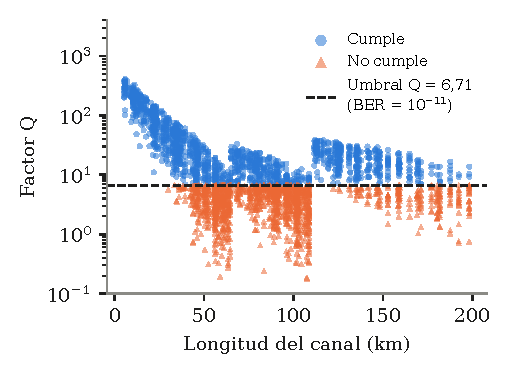
\includegraphics[width=0.7\textwidth]{figuras/fig1_q_vs_longitud}
\caption{Factor Q de cada canal según su longitud (muestra aleatoria de 1500 canales por clase); la línea discontinua es el umbral BER = 10\textsuperscript{−11}.}
\label{fig:q}
\end{figure}

La Tabla~\ref{tab:resultados} recoge las métricas de validación cruzada. En el escenario A, con solo datos de inventario, los tres modelos alcanzan un AUC de 0,98 y un F1 de 0,83–0,85. Al añadir la potencia recibida (escenario B) el AUC sube a 0,998 en los tres modelos y el F1 a 0,93–0,95. El escenario C apenas mejora al B, porque la potencia medida ya recoge casi todo el efecto de las causas ocultas.

\begin{table}[htbp]
\centering
\scriptsize
\caption{Resultados de la validación cruzada estratificada (10 pliegues × 3 repeticiones), media ± desviación típica. Clase positiva: canal que no cumple BER ≤ 10\textsuperscript{−11}.}
\label{tab:resultados}
\begin{tabular}{llcccc}
\toprule
Escenario & Modelo & AUC & Exactitud equilibrada & Sensibilidad & F1 \\
\midrule
A & Regresión logística & 0,983 $\pm$ 0,003 & 0,929 $\pm$ 0,009 & 0,939 $\pm$ 0,017 & 0,832 $\pm$ 0,014 \\
A & Random Forest & 0,981 $\pm$ 0,003 & 0,921 $\pm$ 0,011 & 0,901 $\pm$ 0,023 & 0,847 $\pm$ 0,015 \\
A & XGBoost & 0,982 $\pm$ 0,003 & 0,925 $\pm$ 0,010 & 0,914 $\pm$ 0,019 & 0,845 $\pm$ 0,014 \\
B & Regresión logística & 0,998 $\pm$ 0,001 & 0,977 $\pm$ 0,004 & 0,987 $\pm$ 0,007 & 0,931 $\pm$ 0,009 \\
B & Random Forest & 0,998 $\pm$ 0,001 & 0,976 $\pm$ 0,007 & 0,974 $\pm$ 0,012 & 0,947 $\pm$ 0,012 \\
B & XGBoost & 0,998 $\pm$ 0,001 & 0,973 $\pm$ 0,008 & 0,964 $\pm$ 0,014 & 0,947 $\pm$ 0,012 \\
C & Regresión logística & 0,998 $\pm$ 0,001 & 0,980 $\pm$ 0,004 & 0,991 $\pm$ 0,006 & 0,940 $\pm$ 0,010 \\
C & Random Forest & 0,998 $\pm$ 0,001 & 0,978 $\pm$ 0,006 & 0,976 $\pm$ 0,011 & 0,951 $\pm$ 0,011 \\
C & XGBoost & 0,999 $\pm$ 0,001 & 0,978 $\pm$ 0,007 & 0,969 $\pm$ 0,012 & 0,958 $\pm$ 0,011 \\
\bottomrule
\end{tabular}
\end{table}

La Fig.~\ref{fig:f1} compara el F1 de los tres modelos: la mejora más grande se debe a pasar del escenario A al B, no al cambio de modelo. Dentro de cada escenario, los ensambles superan a la regresión logística en F1 (0,947 frente a 0,931 en B). La prueba de McNemar confirma que, en el escenario B, los ensambles cometen menos errores que la logística (61 frente a 92 de 3000 canales para ambos ensambles): Random Forest acierta 44 canales que la logística falla, frente a 13 en sentido contrario (χ\textsuperscript{2} = 15,79; p = 7\textperiodcentered{}10\textsuperscript{−5}), y XGBoost 54 frente a 23 (χ\textsuperscript{2} = 11,69; p = 6\textperiodcentered{}10\textsuperscript{−4}), ambas significativas tras la corrección de Bonferroni.

\begin{figure}[htbp]
\centering
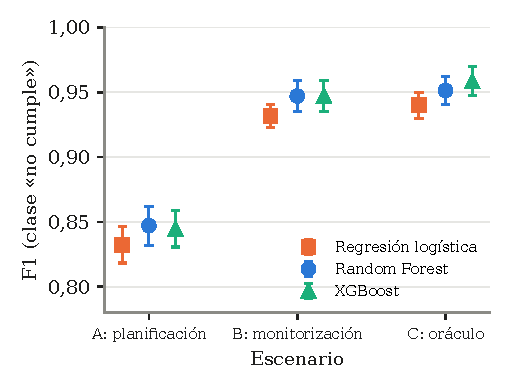
\includegraphics[width=0.7\textwidth]{figuras/fig2_f1_escenarios}
\caption{F1 de la clase «no cumple» por escenario y modelo (media ± desviación típica).}
\label{fig:f1}
\end{figure}

Sin embargo, el AUC y la exactitud equilibrada son prácticamente iguales en los tres modelos, y el tipo de error difiere: en el conjunto de prueba, Random Forest deja sin detectar 12 de los 612 canales que no cumplen y da 49 falsas alarmas, XGBoost 18 y 43, y la regresión logística 2 y 90. Como para el operador un canal defectuoso no detectado cuesta más que una revisión innecesaria, la ventaja del ensamble depende del umbral de decisión y del coste de cada error. En el escenario A no hay una ventaja clara del ensamble (menor AUC y exactitud equilibrada). La hipótesis se confirma, por tanto, con matices.

Los resultados se mantienen fuera de las condiciones de entrenamiento (objetivo 3). Con validación agrupada por trayecto, en el escenario B el AUC es de 0,998, 0,997 y 0,996 y el F1 de 0,931, 0,947 y 0,941 (logística, Random Forest y XGBoost), prácticamente iguales que con la validación estándar; en el escenario A, el F1 es de 0,831, 0,846 y 0,838. Al entrenar con canales de hasta 15 años y evaluar con los más antiguos, el AUC es ≥ 0,991 y el F1 de 0,911, 0,955 y 0,947; al entrenar sin hielo y evaluar por debajo de −5 °C, el AUC es de 0,997 y el F1 de 0,934, 0,949 y 0,942. Las variaciones son pequeñas (hasta unas 0,02 en F1 y sensibilidad). Esta prueba es, no obstante, poco exigente: el simulador no incluye efectos propios de cada trayecto (p. ej., tendidos o climas locales distintos), por lo que la generalización a trayectos reales no vistos debe confirmarse con datos medidos.

La Fig.~\ref{fig:importancia} muestra la importancia de cada variable para Random Forest en el escenario B. Al permutar la potencia recibida el AUC cae 0,26, diez veces más que con la segunda variable (amplificado, 0,03); la temperatura no aporta información. En la red simulada, monitorizar la potencia en el receptor aporta, así, más que cambiar de modelo.

\begin{figure}[htbp]
\centering
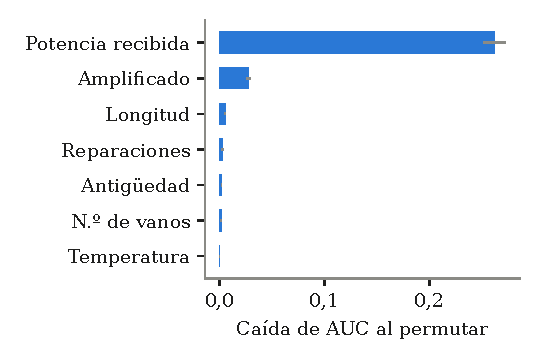
\includegraphics[width=0.7\textwidth]{figuras/fig3_importancia}
\caption{Importancia de las variables por permutación (Random Forest, escenario B). Barras de error: desviación típica en 10 permutaciones.}
\label{fig:importancia}
\end{figure}

Estos resultados concuerdan con la literatura: Random Forest y XGBoost son los clasificadores más precisos en~\cite{kozdrowski2021}, Random Forest también en~\cite{rottondi2018}, y la pérdida de exactitud al reducir variables observada en~\cite{aladin2020} se reproduce aquí al pasar del escenario B al A. Las cifras son más altas que con datos reales~\cite{kozdrowski2021} porque la etiqueta se obtiene de forma determinista de un modelo físico en el que el factor Q depende directamente de la potencia recibida (ecs.~(\ref{eq:2})--(\ref{eq:5})), que el escenario B observa con solo 0,5 dB de error; la importancia de esa variable es, en parte, consecuencia del propio simulador. Esta circularidad y el uso de datos sintéticos son las principales limitaciones del estudio.


\section{Conclusiones}\label{sec:4}

Este trabajo ha construido un modelo físico de la red DWDM ferroviaria Moscú-Kazánskaya – Riazán con degradación en explotación y ha evaluado tres modelos de aprendizaje automático para predecir si cada canal cumple BER ≤ 10\textsuperscript{−11} (objetivos 1 y 2). En el escenario de monitorización (B), los modelos de ensamble cometen significativamente menos errores que la regresión logística (McNemar, p $<$ 0,001 tras Bonferroni) y obtienen mayor F1, de modo que la hipótesis se confirma según el criterio principal, aunque con matices: la ventaja no se extiende a la capacidad de ordenar los canales (AUC de 0,998 en los tres modelos) ni a la detección de canales que no cumplen (sensibilidad 0,987 de la logística frente a 0,974 de Random Forest con el umbral de 0,5), y en el escenario A no hay una ventaja clara. Los resultados se mantienen, en la red simulada, en trayectos, antigüedades y temperaturas no vistos en el entrenamiento (objetivo 3).

En la red simulada, la potencia recibida que ya mide el transceptor es la variable decisiva: con ella cualquiera de los tres modelos supera ampliamente a la estimación con datos de inventario. Como el factor Q se calcula a partir de ella, este resultado debe confirmarse con datos medidos. Como trabajo futuro se proponen la validación con datos de la red real, el ajuste del umbral de decisión según el coste de cada error, la cuantificación del margen de diseño que podría ahorrarse (objetivo 4) y la transferencia de modelos entre redes~\cite{yu2019}.


\bibliographystyle{splncs}
\bibliography{referencias}

\end{document}
